% =============================================================
%  Natural power (surge-impedance loading)
%  Figures in fig/, copied from presentation/design/ac-transmission/fig/
%  (np_*.pdf), generated by that folder's natural_power_figures.py
%  from the exact two-port equations and cross-checked against a
%  20-segment pandapower model (deviation < 0.1 %).
%  Worked line of this section: 400 kV, 2x bundle, 50 Hz, 400 km --
%  not the 500 kV line of Section 6.
% =============================================================
\subsection{Natural Power}
\label{sec:natural-power}

\subsubsection{Definition}
\label{sec:np-definition}

A line terminated in its own wave impedance carries its \emph{natural
power}: the reactive power generated by the shunt capacitance exactly
cancels the reactive power consumed by the series inductance, the line
exchanges no reactive power with either end, and its voltage magnitude stays
constant along the route. North American practice calls the same quantity
the surge-impedance loading, SIL.

On an overhead line $\omega \cdot L' \gg R'$ and $\omega \cdot C' \gg G'$,
so the wave impedance of~\eqref{eq:ac-gamma-zw} is within about a percent of
the real quantity $\sqrt{L'/C'}$, and it is that real value the natural
power is quoted from:
\begin{equation}
  Z_w \approx \sqrt{\frac{L'}{C'}}
  \qquad
  P_{nat} = \mathrm{SIL} = \frac{U^2}{Z_w}
  \label{eq:np-definition}
\end{equation}

$Z_w$ is a property of the conductor geometry alone. It does not depend on
the length of the line, and in the lossless form not on frequency either.
$P_{nat}$ is therefore a reference rather than a rating: below it the line
is a net source of reactive power, above it a net sink.

The same result follows from the two-port equations. Closing the line with
$\underline{Z}_w$ makes $\underline{I}_R = \underline{U}_R /
\underline{Z}_w$, and~\eqref{eq:ac-u-x} and~\eqref{eq:ac-i-x} collapse to a
single travelling wave with no reflection,
\begin{equation}
  \underline{U}(x) = \underline{U}_R \cdot
      e^{\underline{\gamma} \cdot x},
  \qquad
  \underline{I}(x) = \underline{I}_R \cdot
      e^{\underline{\gamma} \cdot x}
  \label{eq:np-matched}
\end{equation}
so that $\underline{U}/\underline{I} = \underline{Z}_w$ everywhere and the
magnitude falls only by the attenuation $e^{-\alpha \cdot l}$,
Figure~\ref{fig:np-matched}. Only the complex $\underline{Z}_w$ matches
perfectly; terminating in the real $\sqrt{L'/C'}$ leaves a small residual
reflection.

\begin{figure}[!ht]
  \centering
  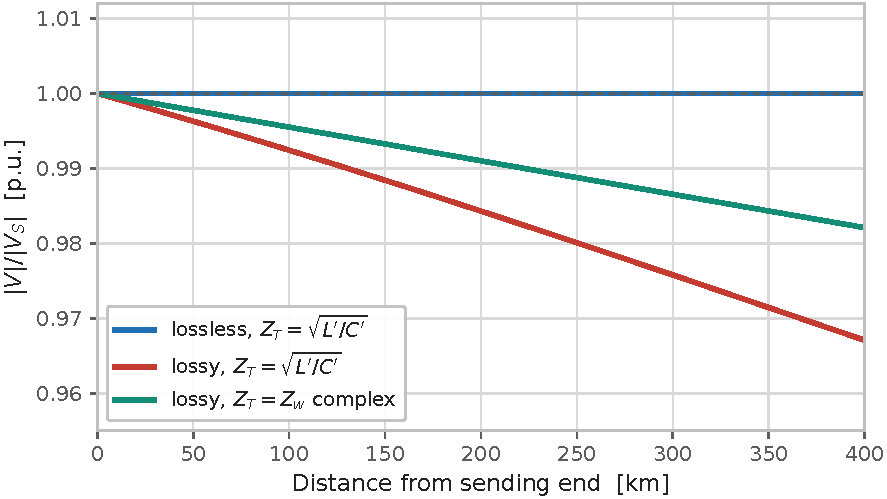
\includegraphics[width=0.78\linewidth]{ac-transmission/fig/np_matched_profile.pdf}
  \caption{Voltage along a line closed in its wave impedance: the profile is
           flat apart from the attenuation, and the residual ripple of the
           real-valued termination}
  \label{fig:np-matched}
\end{figure}

\subsubsection{The reactive balance}
\label{sec:np-balance}

Read as a reactive power balance, a line of length $l$ at line-to-line
voltage $U$ carrying phase current $I$ generates and consumes
\begin{equation}
  Q_C = \omega \cdot C' \cdot l \cdot U^2
  \qquad
  Q_L = 3 \cdot \omega \cdot L' \cdot l \cdot I^2
  \label{eq:np-qcql}
\end{equation}
Natural loading is where the two cancel. Setting $Q_C = Q_L$ eliminates both
$l$ and $\omega$ and gives $I = U / \left(\sqrt{3} \cdot Z_w\right)$, hence
$P_{nat} = \sqrt{3} \cdot U \cdot I = U^2 / Z_w$ again. The cancellation is
independent of length, which is why the natural power is a property of the
cross-section and not of the route.

The worked line of this section is a 400\,kV, 50\,Hz line of 400\,km with a
two-conductor bundle, $R' = 25$\,m$\Omega$/km, $X' = 0.30\,\Omega$/km and
$C' = 12.5$\,nF/km, giving $L' = 0.955$\,mH/km, $Z_w = 276.4\,\Omega$,
$\left|\underline{Z}_w\right| = 276.9\,\Omega$, $\beta \cdot l = 24.88^\circ$
and $P_{nat} = 579$\,MW. It is not the 500\,kV line of
Section~\ref{sec:reference-line}.

Losses move the balance. On the lossless line the zero crossing of the net
reactive flow reproduces $U^2 / Z_w$ to six decimals; on the real line it
falls to 566\,MW, 2.2\,\% below. The sending-end current carries the load
plus the losses, so $3 \cdot I^2 \cdot X' \cdot l$ is larger and the balance
is reached at a lower transfer. Figure~\ref{fig:np-balance} plots the net
reactive flow of both against the transfer.

\begin{figure}[!ht]
  \centering
  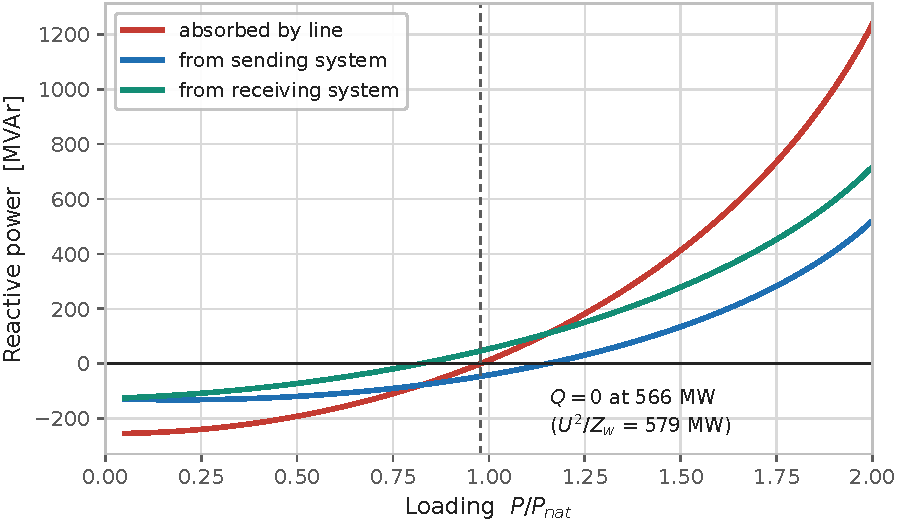
\includegraphics[width=0.78\linewidth]{ac-transmission/fig/np_reactive_balance.pdf}
  \caption{Net reactive power absorbed by the line against transfer,
           $Q_{line} = \Im\left\{\underline{S}_S\right\} -
           \Im\left\{\underline{S}_R\right\}$, lossless and real line}
  \label{fig:np-balance}
\end{figure}

\subsubsection{Voltage profile}
\label{sec:np-profile}

With both terminals held at 1.0\,p.u.\ and the transmission angle solved for
each loading, the profile along the line shows the balance directly,
Figure~\ref{fig:np-profile}. Below $P_{nat}$ the shunt capacitance dominates
and the middle of the line rises, to 1.024\,p.u.\ at no load. At $P_{nat}$
the profile is flat to four decimals. Above it the series reactance
dominates and the middle sags, to 0.873\,p.u.\ at $2 \cdot P_{nat}$, by
which point the angle across the line has reached $63^\circ$.

\begin{figure}[!ht]
  \centering
  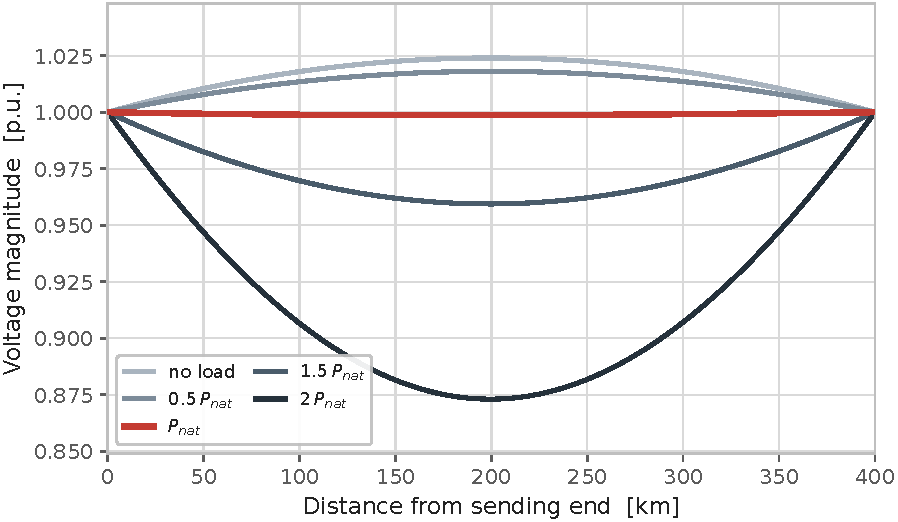
\includegraphics[width=0.78\linewidth]{ac-transmission/fig/np_voltage_profile.pdf}
  \caption{Voltage profile along the 400\,km line at several loadings, both
           terminals at 1.0\,p.u.}
  \label{fig:np-profile}
\end{figure}

\FloatBarrier

\subsubsection{Typical values}
\label{sec:np-typical}

Table~\ref{tab:np-typical} gives the natural power of common line types.

\begin{table}[!ht]
  \centering
  \begin{tabular}{@{}l r r r r r@{}}
    \toprule
    \textbf{Line} & \multicolumn{1}{c}{\textbf{$U$}}
      & \multicolumn{1}{c}{\textbf{$C'$}}
      & \multicolumn{1}{c}{\textbf{$Z_w$}}
      & \multicolumn{1}{c}{\textbf{$P_{nat}$}}
      & \multicolumn{1}{c}{\textbf{$S_{th}/P_{nat}$}} \\
    & \multicolumn{1}{c}{kV} & \multicolumn{1}{c}{nF/km}
      & \multicolumn{1}{c}{$\Omega$} & \multicolumn{1}{c}{MW} & \\
    \midrule
    230\,kV, $1\times$ Drake  & 230 &  9.0 & 376.1 &  141 & 2.8 \\
    345\,kV, $2\times$ bundle & 345 & 11.8 & 292.3 &  407 & 2.6 \\
    400\,kV, $2\times$ bundle & 400 & 12.5 & 276.4 &  579 & 2.4 \\
    500\,kV, $3\times$ bundle & 500 & 13.5 & 256.6 &  974 & 2.3 \\
    765\,kV, $4\times$ bundle & 765 & 13.5 & 250.8 & 2334 & 2.0 \\
    \bottomrule
  \end{tabular}
  \caption{Natural power of typical line types}
  \label{tab:np-typical}
\end{table}

Three things follow. $Z_w$ spans only 251 to 376\,$\Omega$ across the whole
range while $P_{nat}$ spans 141 to 2334\,MW, because $P_{nat}$ is a $U^2$
quantity: voltage, not geometry, sets the transfer. Bundling and tighter
phase spacing are the only levers on $Z_w$, and they work on both terms, 
lowering $L'$ and raising $C'$. And the ratio of thermal rating to natural
power, $S_{th}/P_{nat}$, sets the extent of the thermal plateau of the
loadability curve of Section~\ref{sec:limits}.

AC cables sit at $Z_w \approx 20 \ldots 40\,\Omega$, so their natural power
exceeds the thermal rating and is never reached; as
Section~\ref{sec:cable} sets out, the charging current binds first.

\subsubsection{Light load: the Ferranti effect}
\label{sec:np-ferranti}

On an open-ended line $\underline{I}_R = 0$ and the terminal voltage ratio
follows from~\eqref{eq:ac-abcd-exact} as
\begin{equation}
  \frac{\underline{U}_R}{\underline{U}_S}
    = \frac{1}{\cosh\left(\underline{\gamma} \cdot l\right)}
    \;\longrightarrow\;
    \frac{1}{\cos\left(\beta \cdot l\right)}
  \label{eq:np-ferranti}
\end{equation}
in the lossless limit, so the receiving end rises above the sending end. At
$\beta \cdot l = 24.88^\circ$ the open end reaches 1.102\,p.u., drawing
251\,MVAr of charging power. A 60\,\% shunt reactor brings it back to
0.984\,p.u.; full compensation gives 0.918\,p.u., Figure~\ref{fig:np-ferranti}. The degree of compensation
follows from the light-load voltage, but it also moves the natural power.

\begin{figure}[!ht]
  \centering
  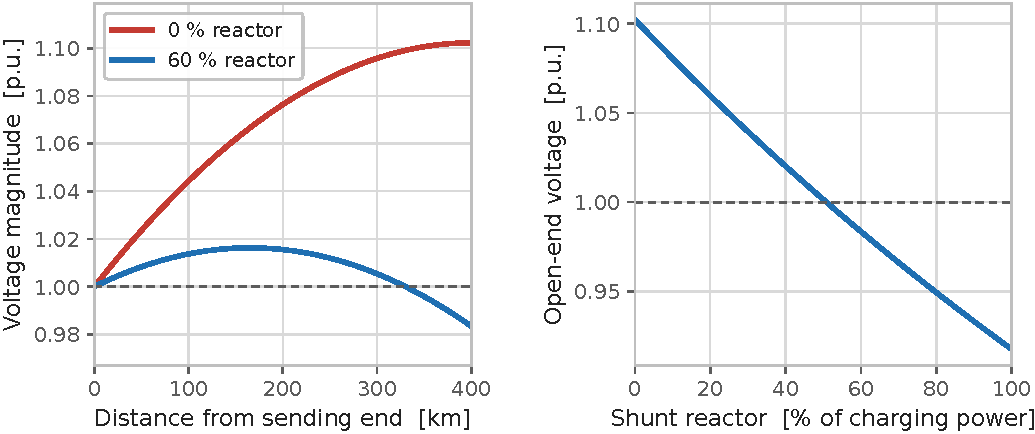
\includegraphics[width=0.74\linewidth]{ac-transmission/fig/np_ferranti.pdf}
  \caption{Open-end voltage rise against line length, and the effect of
           shunt compensation}
  \label{fig:np-ferranti}
\end{figure}

\subsubsection{Effect of compensation on the natural power}
\label{sec:np-compensation}

For uniformly distributed compensation the scaling is exact. Series
compensation of degree $k$ reduces the reactance and shunt compensation of
degree $m$ the capacitance:
\begin{equation}
  X' \to X' \cdot \left(1-k\right)
     \;\Rightarrow\; \frac{P_{nat}}{\sqrt{1-k}},
  \qquad
  C' \to C' \cdot \left(1-m\right)
     \;\Rightarrow\; P_{nat} \cdot \sqrt{1-m}
  \label{eq:np-compensation}
\end{equation}
so $k = 60$\,\% raises $P_{nat}$ by a factor 1.581 and $m = 60$\,\% lowers
it by 0.632, Figure~\ref{fig:np-compensation}.

Real banks are lumped at substations rather than distributed, so these laws
are a first-order guide only. A lumped 30\,\% series bank at $1.4 \cdot
P_{nat}$ on the worked line reduces the transmission angle from $37.6^\circ$
to $25.6^\circ$ and turns the sending-end reactive flow from $+89$ to
$-30$\,MVAr. Section~\ref{sec:series-compensation} treats the lumped case
properly.

\begin{figure}[!ht]
  \centering
  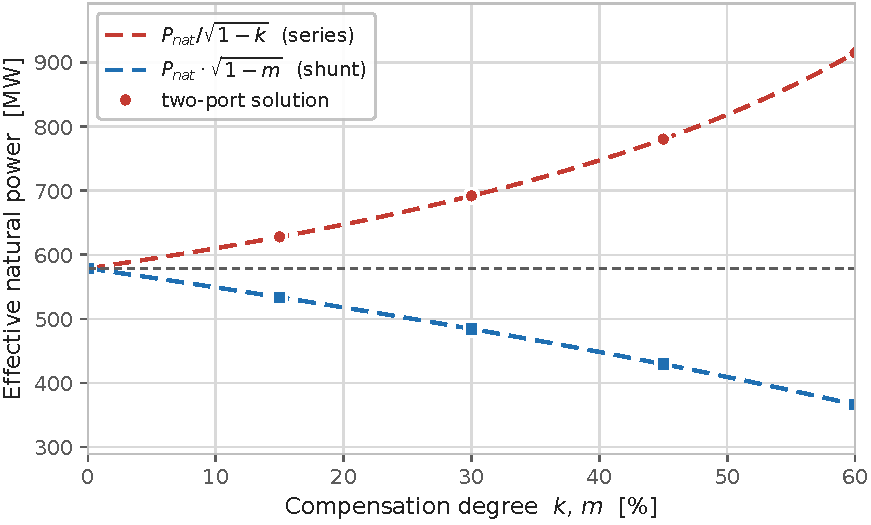
\includegraphics[width=0.74\linewidth]{ac-transmission/fig/np_compensation.pdf}
  \caption{Effect of distributed series and shunt compensation on the
           natural power}
  \label{fig:np-compensation}
\end{figure}

\FloatBarrier
